\documentclass[aspectratio=169]{beamer}

\usetheme{Madrid}
\usepackage{booktabs}
\usepackage{graphicx}
\usepackage{mathtools}

% Drop author/institute from the footer, keep title + date + page number
\setbeamertemplate{footline}{%
  \leavevmode%
  \hbox{%
  \begin{beamercolorbox}[wd=.7\paperwidth,ht=2.25ex,dp=1ex,center]{title in head/foot}%
    \usebeamerfont{title in head/foot}\insertshorttitle
  \end{beamercolorbox}%
  \begin{beamercolorbox}[wd=.3\paperwidth,ht=2.25ex,dp=1ex,leftskip=2ex,rightskip=2ex,sep=0pt]{date in head/foot}%
    \hfill%
    \usebeamerfont{date in head/foot}%
    \insertshortdate{}%
    \hfill%
    \usebeamercolor[fg]{page number in head/foot}%
    \usebeamerfont{page number in head/foot}%
    \usebeamertemplate{page number in head/foot}%
  \end{beamercolorbox}}%
  \vskip0pt%
}

\title{Benchmarking continuous optimization techniques for DAG learning}
\author{Daniele Tarek Iaisy}
\institute{Master's Degree in Artificial Intelligence, University of Bologna}
\date{}

\begin{document}

\maketitle

\section{Introduction}

\begin{frame}{Domain}
    \begin{itemize}
        \item The structure of a Bayesian network can be inferred from data
        \item However, constructing a DAG has a combinatorial cost
        \item This makes it very expensive for networks with many variables
        \item Numerical methods could be applied to get a ``good enough'' solution in reasonable time
    \end{itemize}
\end{frame}

\begin{frame}{Classical algorithms}
    \begin{itemize}
        \item PC\footnote{Spirtes, Glymour, \emph{An Algorithm for Fast Recovery of Sparse Causal Graphs} \cite{spirtes1991pc}} - constraint-based: starts from a fully connected graph and removes edges using conditional independence tests
        \item fGES\footnote{Ramsey, Glymour, Sanchez-Romero, Glymour, \emph{A Million Variables and More: The Fast Greedy Equivalence Search Algorithm for Learning High-Dimensional Graphical Structure of Tetrad} \cite{ramsey2017fges}} - score-based: greedily adds edges to maximize a score, then greedily removes them in a backward phase
        \item The space of possible graphs grows super-exponentially with the number of variables
        \item Main culprit: acyclicity, without it you could fix parents for each node independently, giving a polynomial bound
    \end{itemize}
\end{frame}

\begin{frame}{NOTEARS\footnote{Zheng, Aragam, Ravikumar, Xing, \emph{DAGs with NO TEARS: Continuous Optimization for Structure Learning} \cite{zheng2018dags}}}
    \begin{itemize}
        \item Model the graph as an adjacency matrix $W$
        \item Find a \textbf{smooth} function $h$ s.t. $h(W) = 0 \iff W$ is an acyclic graph
        \item Use the Lagrangian method for constrained optimization on $W$ under the constraint $h(W) = 0$
    \end{itemize}
    \vfill
    \begin{theorem}
        \[ h(W) \coloneqq \mathrm{tr}\left(e^{W \circ W}\right) - d = 0 \iff W \text{ is a DAG} \]
        where $d$ is the number of variables.
    \end{theorem}
\end{frame}

\begin{frame}{DAG-GNN\footnote{Yu, Chen, Gao, Yu, \emph{DAG-GNN: DAG Structure Learning with Graph Neural Networks} \cite{yu2019daggnn}}}
    \begin{itemize}
        \item Builds on NOTEARS
        \item Replaces linear SEM with a VAE using a GNN encoder/decoder
        \item Captures non-linear dependencies
        \item Polynomial constraint for acyclicity
    \end{itemize}
    \vfill
    \begin{theorem}
        For any $\alpha > 0$
        \[ h(W) \coloneqq \mathrm{tr}\left((\mathcal{I}+\alpha W\circ W)^d\right) - d = 0 \iff W \text{ is a DAG} \]
        where $d$ is the number of variables.
    \end{theorem}
\end{frame}

\section{Experiment}

\begin{frame}{Aim}
    \begin{itemize}
        \item Compare classical algorithms against NOTEARS and DAG-GNN
        \item Evaluate how good is the graph reconstructed by each algortihm
        \item Evaluate resource cost and scaling w.r.t. number of variables and dataset size
    \end{itemize}
\end{frame}

\begin{frame}{Method\footnote{Scutari, \emph{Bayesian Network Repository} \cite{bnlearn}}\footnote{Sachs, Perez, Pe'er, Lauffenburger, Nolan, \emph{Causal Protein-Signaling Networks Derived from Multiparameter Single-Cell Data} \cite{sachs2005causal}}}
    \begin{itemize}
        \item Picked 3 networks from the bnlearn repository to generate synthetic dataset + 1 real world dataset
        \item CANCER, 5 nodes discrete variables
        \item CHILD, 20 nodes discrete variables
        \item ALARM, 37 nodes discrete variables
        \item Sachs et al., 11 nodes continuous variables
    \end{itemize}
\end{frame}

\begin{frame}{Results}
    \begin{itemize}
        \item NOTEARS performs really well adding a tolerable overhead
        \item DAG-GNN failed to beat NOTEARS and takes significantly longer
        \item They can scale better to more variables (eg compared to fGES)
        \item They scale worse with a bigger dataset (other algorithms are almost unaffected)
    \end{itemize}
    % TODO: results table / figures
    \begin{table}
        \centering
        \scriptsize
        \begin{tabular}{lrrrrrr}
        \toprule
        Algorithm & Time (s) & nSHD & Cancer & Sachs & Child & Alarm \\
        \midrule
        NOTEARS &  57.27 & 0.90 &  4 & 18 & 21 & 34 \\
        DAG-GNN & 450.88 & 1.00 &  3 & 27 & 24 & 42 \\
        HC      &  10.37 & 1.30 &  3 & 37 & 30 & 61 \\
        PC      &   2.99 & 0.90 &  2 & 30 & 26 & 29 \\
        FGES    &  30.87 & 1.00 &  1 & 26 & 27 & 54 \\
        \bottomrule
        \end{tabular}
    \end{table}
\end{frame}

\begin{frame}{Cancer}
    \centering
    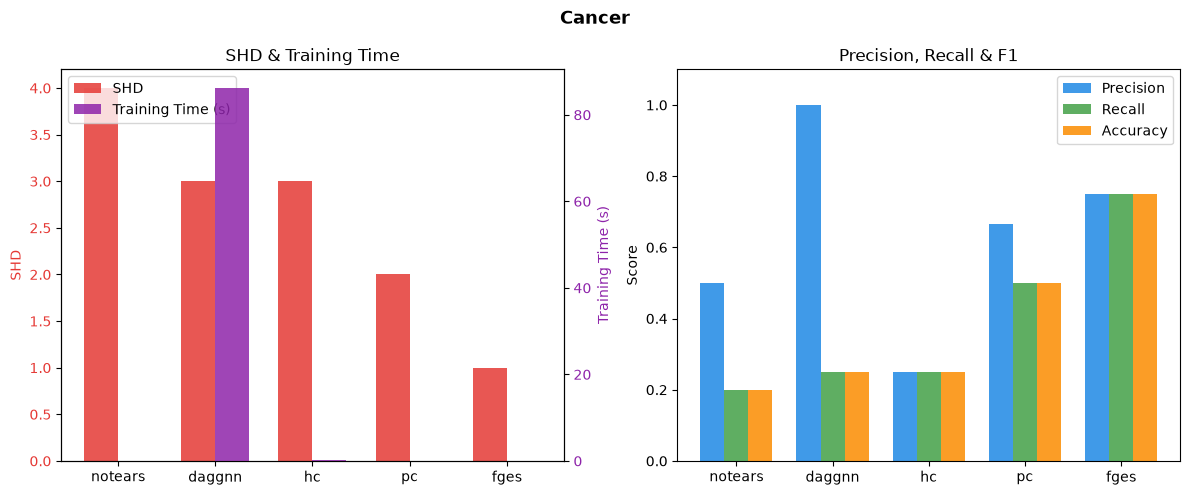
\includegraphics[width=\textwidth,height=0.85\textheight,keepaspectratio]{imgs/cancer.png}
\end{frame}

\begin{frame}{Sachs}
    \centering
    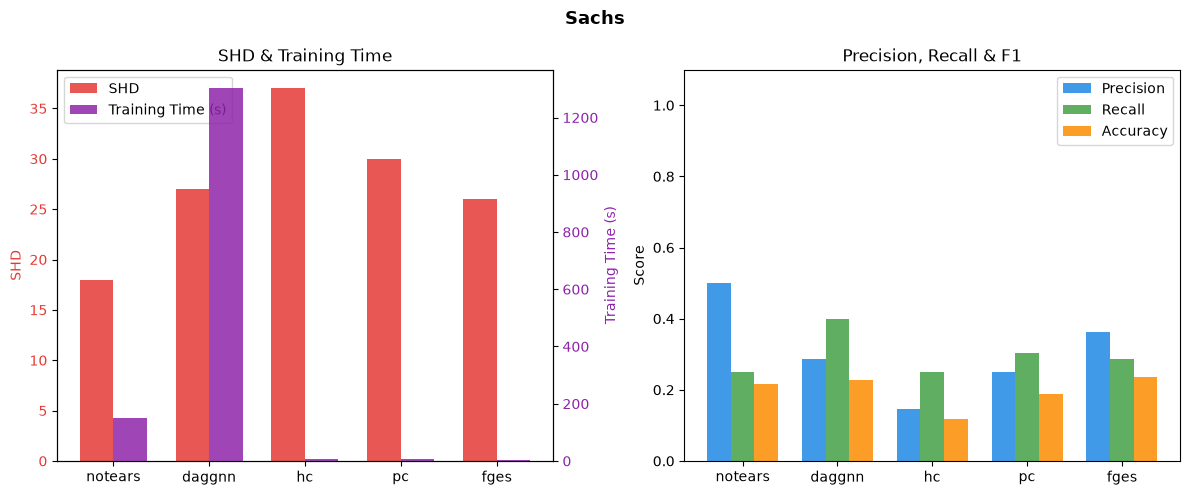
\includegraphics[width=\textwidth,height=0.85\textheight,keepaspectratio]{imgs/sachs.png}
\end{frame}

\begin{frame}{Child}
    \centering
    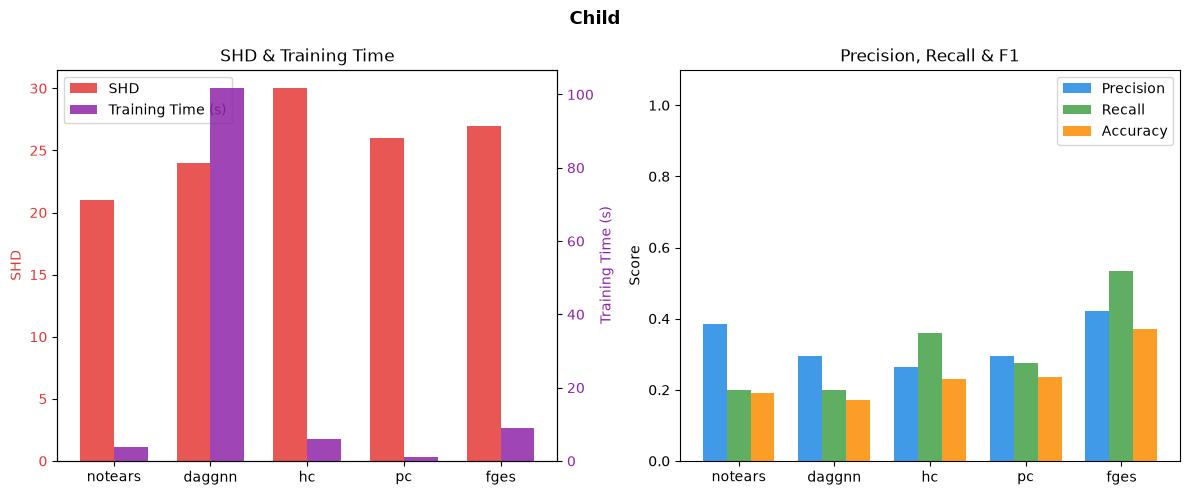
\includegraphics[width=\textwidth,height=0.85\textheight,keepaspectratio]{imgs/child.png}
\end{frame}

\begin{frame}{Alarm}
    \centering
    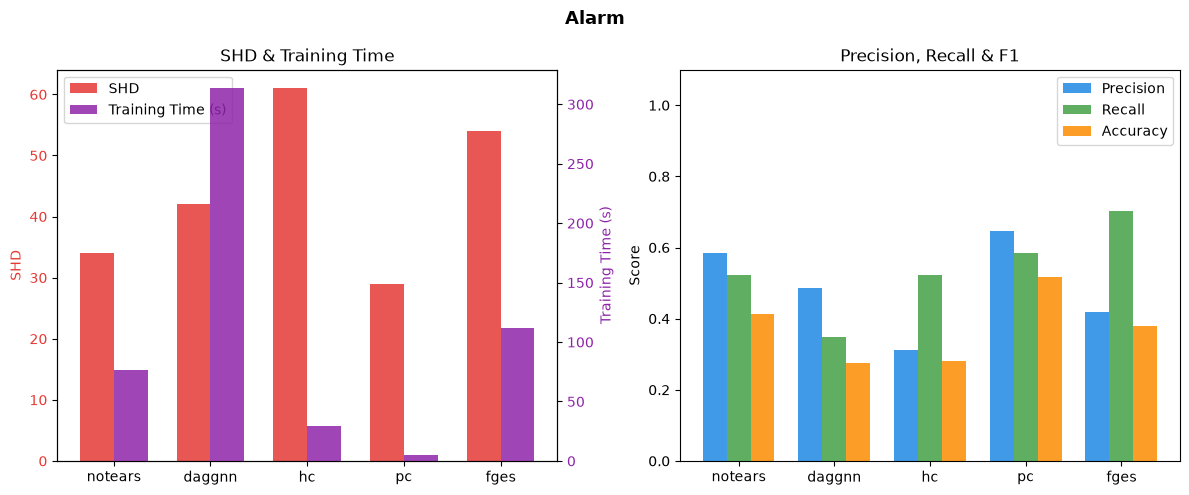
\includegraphics[width=\textwidth,height=0.85\textheight,keepaspectratio]{imgs/alarm.png}
\end{frame}

\begin{frame}{Execution times minus DAG-GNN}
    \centering
    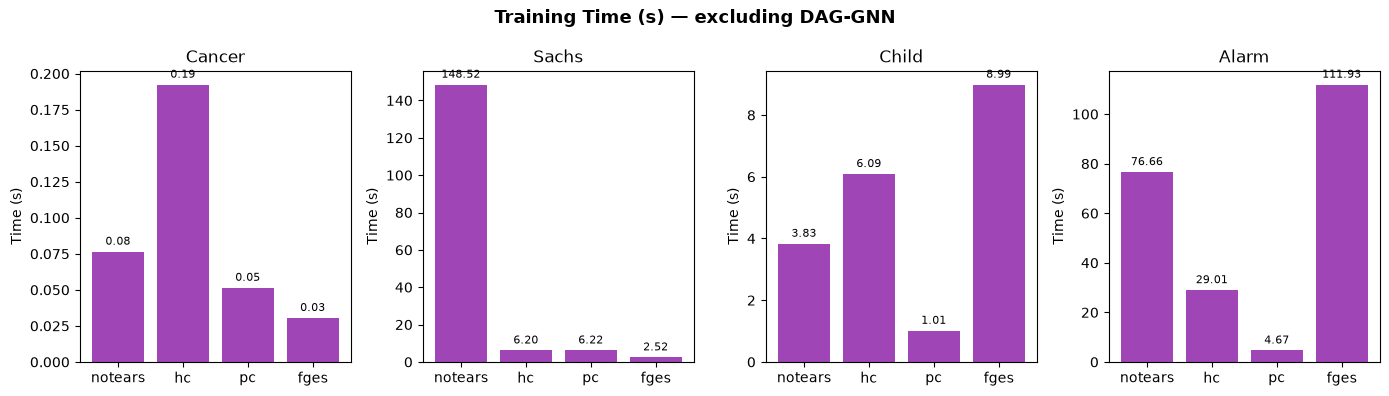
\includegraphics[width=\textwidth,height=0.85\textheight,keepaspectratio]{imgs/times.png}
\end{frame}

\begin{frame}[allowframebreaks]{References}
    \bibliographystyle{plain}
    \bibliography{faikrmod3}
\end{frame}

\end{document}
